%\documentclass[showpacs,superscriptaddress,floatfix,twocolumn,prl]{revtex4}
%\documentclass[11pt,floatfix,notitlepage,amssymb,pra,aps]{revtex4-1}
\documentclass[11pt,floatfix,amssymb,prx,aps,longbibliography,superscriptaddress,nopacs]{revtex4-2}
%\documentclass{amsart}
%\documentclass{report}
%\renewcommand{\familydefault}{cmss}


\usepackage{comment}



%\usepackage[dvipsnames]{xcolor}
\newcommand{\om}{\left( \omega \right)}
\newcommand{\ta}{\tilde{a}\left(\omega\right)}
\newcommand{\tad}{\tilde{a^{\dagger}}\left(\omega\right)}

\newcommand{\tbx}{\tilde{b}_x\left(\omega\right)}
\newcommand{\tbxd}{\tilde{b^{\dagger}}_x\left(\omega\right)}

\newcommand{\tby}{\tilde{b}_y\left(\omega\right)}
\newcommand{\tbyd}{\tilde{b^{\dagger}}_y\left(\omega\right)}


\newcommand{\tZo}{\tilde{Z}\left(\omega\right)}
\newcommand{\tQo}{\tilde{Q}\left(\omega\right)}
\newcommand{\txo}{\tilde{x}\left(\omega\right)}
\newcommand{\tyo}{\tilde{y}\left(\omega\right)}
%\newcommand{\txo}{\tilde{x}_{\scriptscriptstyle{X}}\left(\omega\right)}
%\newcommand{\tyo}{\tilde{x}_{\scriptscriptstyle{Y}}\left(\omega\right)}
\newcommand{\tNx}{\tilde{N}_x\left(\omega\right)}
\newcommand{\tNy}{\tilde{N}_y\left(\omega\right)}
\newcommand{\tNi}{\tilde{N}_i\left(\omega\right)}
\newcommand{\ccm}{\chi_\mathrm{c}^-\left(\omega\right)}
%\newcommand{\cxm}{\chi_x^-\left(\omega\right)}
%\newcommand{\cym}{\chi_y^-\left(\omega\right)}
\newcommand{\cxm}{\chi_x\left(\omega\right)}
\newcommand{\cym}{\chi_y\left(\omega\right)}
\newcommand{\Ix}{\tilde{I}_x\left(\omega\right)}
\newcommand{\Iy}{\tilde{I}_y\left(\omega\right)}

%\newcommand{\Vm}{\boldmath{V}^{\scriptscriptstyle{\mathrm{M}}}}
\newcommand{\Vm}{V^{\scriptscriptstyle{\mathrm{M}}}}
\newcommand{\nm}{\bar{n}}
\newcommand{\nX}{n_{\scriptstyle{x}}}
\newcommand{\nY}{n_{\scriptstyle{y}}}
\newcommand{\OmegaXY}{\Omega_{\scriptstyle{x,y}}}
\newcommand{\OmegaX}{\Omega_{\scriptstyle{x}}}
\newcommand{\OmegaY}{\Omega_{\scriptstyle{y}}}
\newcommand{\OmegaZ}{\Omega_{\scriptstyle{z}}}
\newcommand{\Omegab}{\Omega_{\mathrm{b}}}
\newcommand{\Omegad}{\Omega_{\mathrm{d}}}
\newcommand{\Omegaeff}{\Omega_{\scriptstyle{\mathrm{eff}}}}
\newcommand{\GY}{\Gamma_{\scriptstyle{y}}}
\newcommand{\GX}{\Gamma_{\scriptstyle{x}}}
\newcommand{\GXY}{\Gamma_{\scriptstyle{x,y}}}
\newcommand{\omegaL}{\omega_{\scriptscriptstyle{\mathrm{L}}}}
\newcommand{\gX}{g_{\scriptstyle{x}}}
\newcommand{\gY}{g_{\scriptstyle{y}}}
\newcommand{\gb}{g_{\mathrm{b}}}
\newcommand{\bX}{\hat{b}_{\scriptstyle{x}}}
\newcommand{\bY}{\hat{b}_{\scriptstyle{y}}}
\newcommand{\bdX}{\hat{b}^{\dagger}_{\scriptstyle{x}}}
\newcommand{\bdY}{\hat{b}^{\dagger}_{\scriptstyle{y}}}
\newcommand{\ac}{\hat{a}_{\mathrm{c}}}
\newcommand{\Gm}{\Gamma_{\mathrm{m}}}
\newcommand{\Omegamj}{\Omega_{j}}
\newcommand{\xzpf}{x_{\mathrm{zpf}}}
\newcommand{\pzpf}{p_{\mathrm{zpf}}}
\newcommand{\yzpf}{y_{\mathrm{zpf}}}
\newcommand{\Xc}{\mathrm{X}_{\scriptstyle{\mathrm{c}}}}
\newcommand{\Yc}{\mathrm{Y}_{\scriptstyle{\mathrm{c}}}}
%\newcommand{\xX}{x_{\scriptscriptstyle{X}}}
%\newcommand{\xY}{x_{\scriptscriptstyle{Y}}}
%\newcommand{\pX}{p_{\scriptscriptstyle{X}}}
%\newcommand{\pY}{p_{\scriptscriptstyle{Y}}}
\newcommand{\xX}{x}
\newcommand{\xY}{y}
\newcommand{\pX}{p_{\scriptstyle{x}}}
\newcommand{\pY}{p_{\scriptstyle{y}}}
\newcommand{\ud}{\mathrm{d}}
\newcommand{\blu}[1]{{\color[rgb]{0,0,1}#1}}
\newcommand{\rosso}[1]{{\color[rgb]{1,0,0}#1}}
\newcommand{\verde}[1]{{\color[rgb]{0,1,0}#1}}
\newcommand{\viola}[1]{{\color[rgb]{1,0,1}#1}}

%\newcommand{\xiX}{\xi_{\scriptscriptstyle{X}}}
%\newcommand{\xiY}{\xi_{\scriptscriptstyle{Y}}}
\newcommand{\xiX}{\xi_{\scriptstyle{x}}}
\newcommand{\xiY}{\xi_{\scriptstyle{y}}}

\newcommand{\supp}{s}
\newcommand{\splitt}{\delta}
\newcommand{\cor}{c}

\usepackage{amsmath}
\usepackage[dvips]{graphicx}
\usepackage{epsfig}
\usepackage{tabularx}
\pagestyle{plain}
\usepackage{lineno}
\usepackage{ulem}
\usepackage{xcolor}
\usepackage{soul}
%\linespread{1.6}


\begin{document}


\title{High purity two-dimensional levitated mechanical oscillator}

\author{Q. Deplano}
\email{These authors contributed equally}
\affiliation{Dipartimento di Fisica e Astronomia, Universit\`a di Firenze, via Sansone 1, I-50019 Sesto Fiorentino (FI), Italy}
\affiliation{INFN, Sezione di Firenze, via Sansone 1, I-50019 Sesto Fiorentino (FI), Italy}

\author{A. Pontin}
\email{These authors contributed equally}
\affiliation{CNR-INO, largo Enrico Fermi 6, I-50125 Firenze, Italy}

\author{A. Ranfagni}
\affiliation{Dipartimento di Fisica e Astronomia, Universit\`a di Firenze, via Sansone 1, I-50019 Sesto Fiorentino (FI), Italy}

\author{F. Marino}
\affiliation{CNR-INO, largo Enrico Fermi 6, I-50125 Firenze, Italy}
\affiliation{INFN, Sezione di Firenze, via Sansone 1, I-50019 Sesto Fiorentino (FI), Italy}

\author{F. Marin}
\email[Electronic mail: ]{francesco.marin@unifi.it}
\affiliation{Dipartimento di Fisica e Astronomia, Universit\`a di Firenze, via Sansone 1, I-50019 Sesto Fiorentino (FI), Italy}
\affiliation{European Laboratory for Non-Linear Spectroscopy (LENS), via Carrara 1, I-50019 Sesto Fiorentino (FI), Italy}
\affiliation{INFN, Sezione di Firenze, via Sansone 1, I-50019 Sesto Fiorentino (FI), Italy}
\affiliation{CNR-INO, largo Enrico Fermi 6, I-50125 Firenze, Italy}

%\date{\today}

\begin{abstract}
In recent years, levitated optomechanics has delivered on the promise of reaching the motional quantum ground state. An important next milestone of the field would be the generation of mechanical entanglement. An ideal candidate is the two-dimensional motion in the polarization plane of an optical tweezer inside an optical cavity, where optical and mechanical modes are coupled via coherent scattering. Achieving this goal requires two key conditions: two-dimensional ground state cooling along with substantial spectral overlap between the two modes. The latter is essential to generate the necessary correlations, but unfortunately, it hinders efficient cooling thus narrowing the useful parameter space. In this work, we report the achievement of a high purity two-dimensional state in a regime where the strong optomechanical coupling induces the desired spectral overlap between oscillations in different directions, as reflected in the non-trivial spectral shape of the detected cavity field. As a result, significant correlations consistently arise between any pair of orthogonal directions, preventing the motion from being reduced to two independent one-dimensional oscillators and leading to higher purity compared to that scenario. Our system serves as an excellent platform for realizing continuous variable entanglement in two-dimensional motion.


\end{abstract}

\maketitle

\section*{Introduction}
Levitated optomechanical systems provide a powerful platform for the manipulation of mesoscopic quantum objects with applications ranging from fundamental physics~\cite{Li2010,Moore2022,Gratta2014} to quantum sensing~\cite{Geraci2010,Tania2024} and technologies~\cite{Vinante2024}. Some of these systems have been cooled near the zero-point energy~\cite{Delic2020,Ranfagni2022,Piotrowski2023,Magrini2021,Tebbenjohanns2021} opening the way towards more refined quantum experiments including the preparation of novel quantum states~\cite{RomeroIsart2024,Neumeier2024,Nothup2024,Frimmer2024} and tests of the quantised nature of gravity~\cite{Bose2017}.

The motion of a levitated nanoparticle in the transverse plane of a tightly focused laser beam (optical tweezer \cite{Ashkin1970}) in high vacuum \cite{Millen2020,Gonzalez-Ballestero2021} offers a valuable opportunity to realise a two-dimensional oscillator with quantum properties. The optical potential generated by the tweezer light is proportional to its intensity, whose profile has an elliptical shape near the focus. In the transverse plane it is well approximated by a paraboloid that defines two orthogonal axes to which different natural frequencies of the oscillatory motion of the nanoparticle are associated. We will call them $X$ and $Y$ axes. The axis corresponding to the tighter focusing direction ($X$), providing the highest oscillation frequency, is typically orthogonal to the main polarization axis of the tweezer \cite{Novotny2012}. 

By placing the levitated particle inside an optical cavity with a suitable resonance frequency, a mode of the cavity field is populated by the scattered tweezer light. The oscillatory motion of the nanoparticle is coupled to the cavity field via this coherent scattering \cite{Vuletic2000,Windey2019,Delic2019A,Quidant2020}. When the particle is positioned on a node of the cavity standing wave, it is precisely the motion along the cavity axis ({\it bright mode}) that is coupled to the cavity field \cite{Toros2020B,Toros2021,Borkje2023}. Consequently, the $X$ and $Y$ oscillations have optomechanical coupling rates proportional to $\sin \theta$ and $\cos \theta$ respectively, where $\theta$ is the angle between the $Y$ direction and the cavity axis, which is assumed to be orthogonal to the tweezer axis. If $\theta$ is close to $90^{\circ}$, the $X$ oscillation can be optically cooled very efficiently by red detuning the tweezer light with respect to the cavity resonance. Thermal occupancies below unity \cite{Delic2020} (as low as 0.5 \cite{Ranfagni2022,Piotrowski2023}) have actually been achieved. On the other hand, an angle $\theta$ close to $45^{\circ}$ allows to obtain significant optomechanical coupling and cooling for both the $X$ and the $Y$ motion. If the two mechanical resonances remain well separated with respect to their width, which is enhanced by the optomechanical damping, the planar motion can still be considered as the sum of two independent mechanical modes, which could be jointly cooled near \cite{Ranfagni2022} and even both below \cite{Piotrowski2023} unity occupation number. 

If the two eigenfrequencies are close to each other, the full potential of a two-dimensional quantum system emerges thanks to the spectral overlap of the $X$ and $Y$ modes. For instance, it enabled the observation of vectorial polaritons \cite{Ranfagni2021} and the cancellation of the quantum backaction \cite{Ranfagni2023}. On the other hand, two-dimensional cooling becomes more difficult because the motion orthogonal to the cavity axis ({\it dark mode}) is not directly coupled to the optical field, but it is simply sympathetically cooled by the bright mode \cite{Toros2021} with a rate proportional to the difference between the two eigenfrequencies.   

In this work, we push the optical cooling of the two-dimensional motion of a levitated nanosphere close to the ground state (i.e., achieving thermal occupancy well below unity in all directions) by going beyond the optomechanical weak-coupling regime. By maintaining significant spectral overlap between the $X$ and $Y$ modes we ensure that they both largely share the same bath, in which quantum fluctuations play a major role. 

The resulting correlations are a fundamental characteristic of our two-dimensional dynamics, which cannot be simply decomposed into the sum of independent orthogonal oscillations.

As a first indicator of quantumness, we calculate the global state purity. We show that, thanks to the correlation between $X$ and $Y$, its value is significantly greater than the simple $ 1/(2\nX + 1)(2 \nY +1) $ attained by independent oscillators having the thermal occupancies $\nX$ and $\nY$. This indicates the enhanced quantumness of the system. To quantify this further, we evaluate the quantum discord, i.e., the quantum component of the mutual information between the two oscillators, and show that it is indeed significantly greater than zero. The two high purity oscillators then also exhibit quantum correlations and thus provide an important platform for applications in quantum information and sensing.

\section*{Experiment}

A $100\,$nm silica nanosphere is loaded onto an optical tweezer in a first chamber under low vacuum conditions, then transferred to a second tweezer in the science chamber at a pressure of about $10\,$mbar \cite{Calamai2021}. The science tweezer is based on $250\,$mW light power generated by a Nd:YAG NPRO laser at $1064\,$nm. A doublet of aspheric lenses, with focal lengths of $18.4\,$mm and $3.1\,$mm respectively, collects the light from a polarization maintaining fiber and refocuses it with a waist narrower than $1\,\mu$m. This optical system can be positioned with nanometric precision inside an optical cavity whose optical axis is orthogonal (within $\sim 1^{\circ}$) to the axis of the tweezer. The light is linearly polarized along a direction at $\sim 45^{\circ}$ with respect to the cavity axis (Fig. \ref{Fig1}). The oscillation frequencies of the nanosphere in the optical potential are, respectively, $(\OmegaX, \OmegaY, \OmegaZ)/2\pi = (121.1,108.5,21.4)\,$kHz for the $(X, Y, Z)$ axes.
\begin{figure}[!htb]
    \centering
    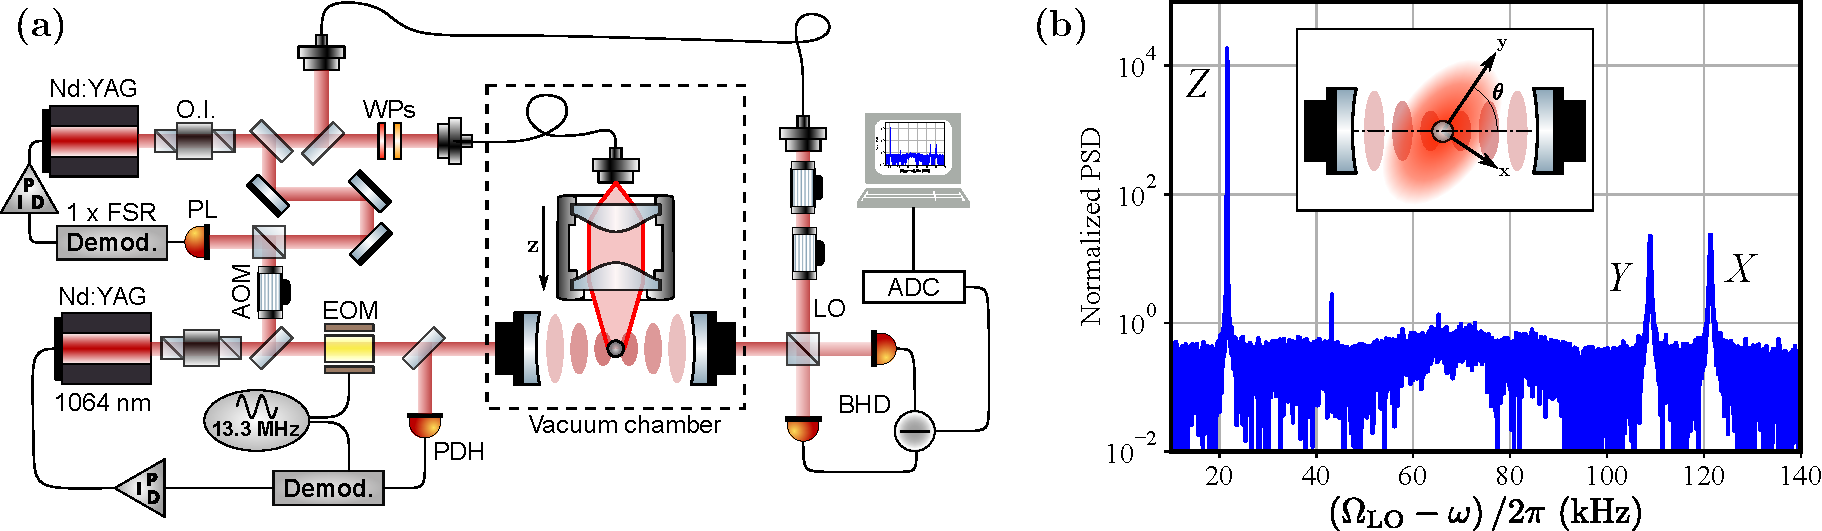
\includegraphics[scale=0.5]{fig1_v3.pdf}
    \caption[Fig1]{\textbf{Overview of the experiment}. a) Simplified scheme of the experimental setup. OI: optic isolator, WP: wave plate, PL: phase locking photodiode, AOM: acousto-optic modulator, EOM: electro-optic modulator, PDH: Pound-Drever-Hall detection, LO: local oscillator, BHD: balanced heterodyne detection, ADC: analog-to-digital converter. b) Power spectral density (PSD) of the heterodyne signal for a detuning $\Delta/2\pi = -250\,$kHz. We show the anti-Stokes sideband, and we report in the abscissa $(\Omega_{\mathrm{LO}}-\omega)/2\pi$. The spectrum is normalized to the measured shot noise which is then subtracted (the dark noise, which is $\sim10\,$dB lower than the shot noise, is preliminarily subtracted from all spectra).
    %The electronic noise is subtracted from the spectrum (it is about $10\,$dB lower than the shot noise of the local oscillator), and the result is normalized to the measured shot noise, obtained by blocking the signal field. Then, the shot noise, equal to $1$, is subtracted as well.
    The three resonance peaks corresponding to the $X$, $Y$ and $Z$ modes are identified. The inset shows the scheme of a plane orthogonal to the tweezer axis, where $Y$ denotes the tweezer polarization axis, and $X$ its orthogonal direction.}
    \label{Fig1}
\end{figure}

The optical cavity has a linewidth of $\kappa/2\pi = 57\,$kHz (full width at half maximum) and it is made with a pair of equal concave mirrors in a nearly concentric configuration, giving a free-spectral-range of $\mathrm{FSR} = 3.07\,$GHz. An auxiliary Nd:YAG
laser is frequency-locked to the optical cavity, while the tweezer laser is phase-locked to the auxiliary laser with a tunable frequency offset equal to $\mathrm{FSR} + \Delta/2\pi$. This setup precisely determines the detuning $\Delta$ of the tweezer radiation from a cavity resonance. 
The light scattered into the cavity mode and transmitted through the end mirror is analyzed using a balanced heterodyne detection. 

After the transfer, the tweezer light is red detuned with respect to a cavity resonance, the nanoparticle is positioned on the cavity axis in correspondence of a node of the standing wave, and the science chamber is pumped down to a pressure of about $3\times10^{-8}\,$mbar. 

The spectrum of the heterodyne signal, normalized to shot noise, can be expressed as
\begin{equation}
S_{\mathrm{out}}(\Omega_{\scriptscriptstyle{\mathrm{LO}}}+\omega) 
= 1 + \eta \,\kappa \,\left|\chi_\mathrm{c}\left(\omega\right)\right|^2 \,\gb^2 \,S_{x_\mathrm{b} x_\mathrm{b}}\om
\label{eq_Sout}
\end{equation}
where 
$\Omega_{\scriptscriptstyle{\mathrm{LO}}}$ is the angular frequency of the local oscillator (in our experiment, we set $\Omega_{\scriptscriptstyle{\mathrm{LO}}}/2\pi = 900\,$kHz using two consecutive AOMs, working on opposite orders to blue-shift the local oscillator beam), $\eta$ is the overall detection efficiency, and $\gb$ is the optomechanical coupling rate for the motion along the cavity axis. 
%defined in terms of the $X$ and $Y$ frequencies and coupling rates by 
%$\gb = \sqrt{(\gX^2\OmegaX+\gY ^2 \OmegaY)/\Omega_{b}}$ and
%$\Omega_{b}=\sqrt{(\gX^2 \OmegaX^3+\gY^2 \OmegaY^3)/(\gX^2\OmegaX+\gY^2 \OmegaY)}$. 
The displacement spectrum $S_{x_\mathrm{b} x_\mathrm{b}}$ of the bright mode appears filtered by the optical susceptibility $\chi_\mathrm{c}(\omega)=\left[-i(\Delta+\omega)+ (\kappa/2)\right]^{-1}$. It can be written as \cite{SM1}:
%\begin{multline}
%S_{x_\mathrm{b} x_\mathrm{b}}\om=\frac{1}{\gb^2}
%\frac{4}{\left|1-2 i \chi_\mathrm{c}^{-}
%\left(\gX^2 \chi_x+\gY^2 \chi_y\right)\right|^2}  \\
%\Bigr[\gX^2 \GX \left|\chi_x\right|^2
%+ \\
%+\gY^2 \GY\left|\chi_y\right|^2+\left|\gX^2 \chi_x+\gY^2 \chi_y\right|^2
%\kappa \left|\chi_\mathrm{c}\left(-\omega\right)\right|^2\Bigr].
%\label{eq:Sxb}
%\end{multline}
\begin{equation}
S_{x_\mathrm{b} x_\mathrm{b}}\om=\frac{4}{\gb^2}\,
\frac{\gX^2 \,\GX \left|\chi_x(\omega)\right|^2
+\gY^2 \,\GY\left|\chi_y(\omega)\right|^2+\left|\gX^2 \chi_x(\omega)+\gY^2 \chi_y(\omega)\right|^2
\kappa \left|\chi_\mathrm{c}\left(-\omega\right)\right|^2}
{\left|1-2 i \chi_\mathrm{c}^{-}\left(\gX^2 \chi_x(\omega)+\gY^2 \chi_y(\omega)\right)\right|^2}
\label{eq:Sxb}
\end{equation}
where we have defined $\chi_{c}^{-}=\chi_{c}\om - \chi_{c}^*\left(-\omega\right)$ and the mechanical susceptibilities are $\chi_{j}\om=\Omegamj \left[\Omegamj^2-\omega^2-i \gamma_{j} \omega\right]^{-1}$ (with $j = x, y$). $\gamma_j$, $g_j$ and $\Gamma_j$ are respectively the rates of gas damping, optomechanical coupling, and decoherence.

In Fig. \ref{Fig1}b we display an example of such a spectrum, acquired for a detuning of $\Delta/2\pi = -250\,$kHz. The oscillations along the $X$ and $Y$ axes, projected along the cavity axis, produce two clear peaks, broadened and shifted by the optomechanical coupling.
With the detuning closer to the mechanical frequencies, both modes are cooled and broadened more effectively, so that their spectra largely overlap. This is clearly visible in the heterodyne spectrum displayed in Fig. \ref{Fig2}, which is acquired at a detuning of $\Delta/2\pi = -111\,$kHz. 

\section*{Discussion}

In Fig. \ref{Fig2}a we show that the model yielding Eqs. (\ref{eq_Sout}-\ref{eq:Sxb}) well fits the experimental data in a wide frequency range where the heterodyne spectrum is dominated by the motion in the $X-Y$ plane. Outside this region, the narrow peak given by the much warmer $Z$ motion is clearly visible around $21\,$kHz, as well as broader structures due to erratic frequencies of the rotational motion~\cite{Barker2023,Ulbricht2018}. The theoretical curve fitted to the right (anti-Stokes) sideband well reproduces also the weaker left sideband. This confirms the validity of the independently measured parameters, in particular the detection efficiency $\eta$ which plays a crucial role in our evaluation of the decoherence rates and consequently of the thermal occupancies and state purity.   

In the numerator of Eq. (\ref{eq:Sxb}), we can identify the contributions of the classical noise sources acting on the $X$ and $Y$ oscillators, quantified by the decoherence rates $\Gamma_j$, and of the quantum bath provided by
the optical vacuum noise. In Figs. \ref{Fig2}b-c we highlight that all three noise sources yield relevant and distinct contributions to the spectral shape. It is therefore clear that measuring the projection on the cavity axis is sufficient to fully characterize the two-dimensional motion. Its relevant parameters, deduced from the fit, are reported in Table \ref{tab_parametri}. 

%\begin{table}
%\begin{tabular}{c|c}
%  $\OmegaX/2\pi$ (Hz)  &  %$122170\pm120$  \\
%   $\OmegaY/2\pi$ (Hz)   &  %$109370\pm150$ \\
% $\gX/2\pi$ (Hz)    & $14130\pm220$ \\
%   $\gY/2\pi$ (Hz)   &  $10370\pm160$  \\
% $\GX/2\pi$ (Hz)    &  $4030\pm200\pm120$  \\
%  $\GY/2\pi$ (Hz)    & $3050\pm170\pm90$  \\
%\end{tabular}
%\end{table}

\begin{table}
\begin{tabular}{|c|c|c|c|c|c|}
\hline
  $\OmegaX/2\pi$ (Hz)  &  
   $\OmegaY/2\pi$ (Hz)   & 
 $\gX/2\pi$ (Hz)    & 
   $\gY/2\pi$ (Hz)   &  
 $\GX/2\pi$ (Hz)    &  
  $\GY/2\pi$ (Hz)     \\
  \hline
  $\,122170\pm120\,$     &  $\,109370\pm150\,$    & $\,14130\pm220\,$    &  $\,10370\pm160\,$   &  $\,4030\pm200\pm120\,$   & $\,3050\pm170\pm90\,\,$  \\
    \hline
\end{tabular}
\caption{Parameters extracted from the fit of of the heterodyne spectrum (left sideband) with the model of Eqs. (\ref{eq_Sout}-\ref{eq:Sxb}). The reported uncertainty is the spread (one standard deviation) on five independent acquisitions. For the decoherence rate, the second quoted error is due to an uncertainty of $5\%$ in the detection efficiency, whose independent measurement yields $\eta = 0.32$.}
\label{tab_parametri}
\end{table}

We remark that the spectral contributions due to classical noise are frequency symmetric in $S_{x_\mathrm{b} x_\mathrm{b}}$, and differ in the two sidebands of $S_{\mathrm{out}}$ only due to cavity filtering. In contrast, quantum noise is present almost exclusively in the Stokes motional sideband where, in our experiment, it largely overwhelms classical noise. This produces markedly different shapes in the two sidebands, a feature that is a clear signature of quantum two-dimensional motion \cite{Ranfagni2023} and testifies to the low effective temperature achieved.
\begin{figure}[!htb]
    \centering
%    \includegraphics[scale=0.6]{budget_bbd.png}
      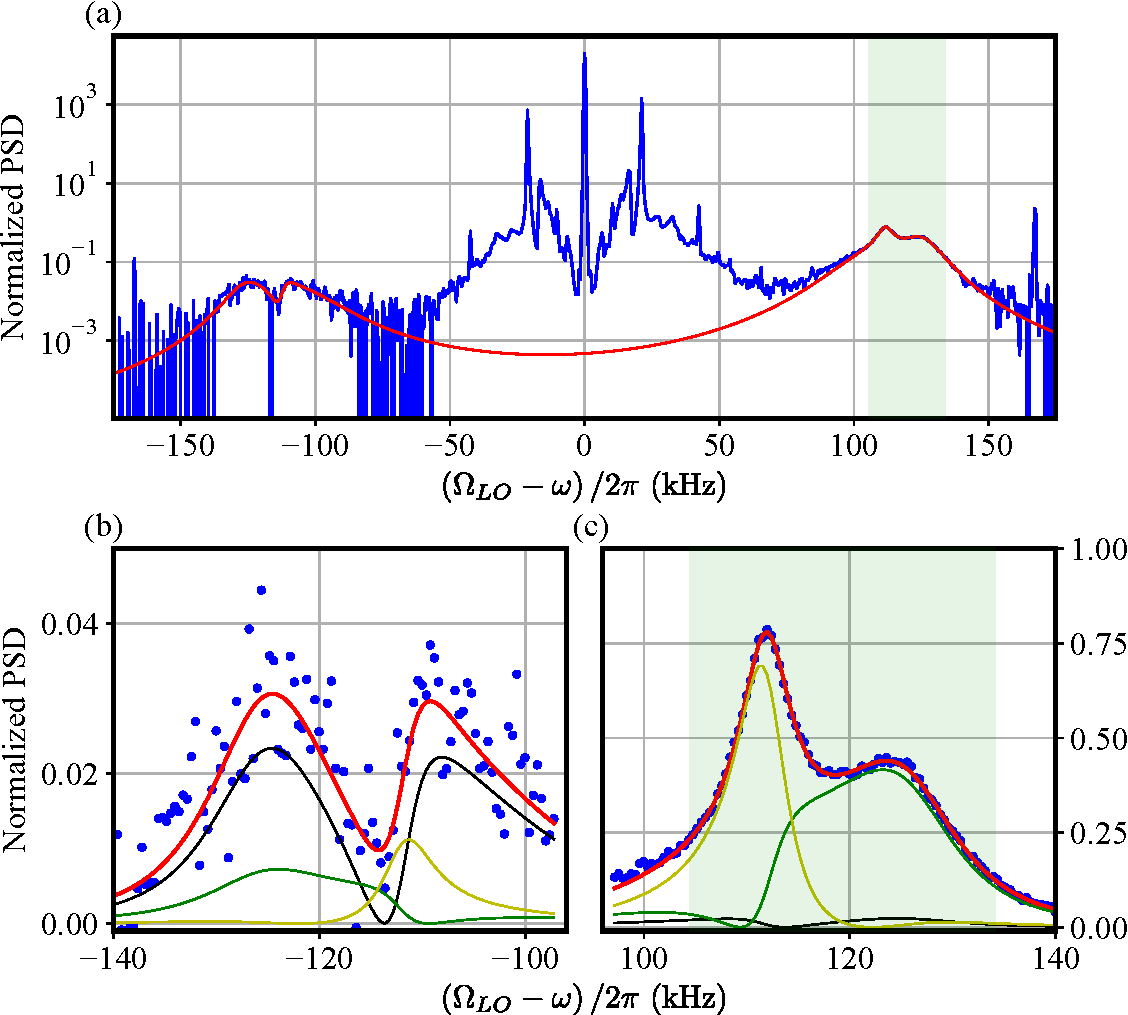
\includegraphics[scale=0.65]{figure_542-652_v4.pdf}
    \caption[Fig2]{\textbf{Power Spectral Density of the heterodyne signal}. The spectrum is normalized to the measured shot noise which is then subtracted (the dark noise is preliminarily subtracted from all spectra). The abscissa is the frequency difference with respect to the local oscillator. The detuning is $\Delta/2\pi = -111\,$kHz. The red solid line shows the fit of Eqs. (\ref{eq_Sout}-\ref{eq:Sxb}) to the experimental anti-Stokes sideband (the spectral region used for the fit is shaded). The lower panels display enlarged views of the left (b) and right (c) sidebands, where different contributions to the fitted curves are shown in dark green (term $\propto \GX$), yellow (term $\propto \GY$), and black (quantum noise, term proportional to $\kappa$).}
    \label{Fig2}
\end{figure}

The quantum steady state of the optomechanical system is characterized by its covariance matrix $V_{ij} = 0.5\langle \{u_i , u_j\} \rangle$ where $u^T = (Q,\,  P,\, \xX,\, \pX,\, \xY,\, \pY)$, $P$ and $Q$ are the two quadratures of the intracavity field, $\xX$ and $\xY$ are the positions and $\pX$ and $\pY$ the momenta of the $X$ and $Y$ oscillators normalized to the respective zero-point fluctuations. The covariance matrix can be calculated using the Lyapunov equation $\,AV+VA^T = -D$ with the drift matrix 
\begin{equation}
    A=
    \left(
    \begin{array}{cccccc}
        -\kappa/2 & -\Delta & 0  & 0 & 0  & 0 \\
         \Delta & -\kappa/2 & 2 \gX  & 0 & 2 \gY  & 0 \\
         0 & 0 & 0  & \OmegaX & 0  & 0 \\
         2 \gX & 0 & -\OmegaX  & -\gamma_x & 0  & 0 \\
         0 & 0 & 0  & 0 & 0  & \OmegaY \\
         2 \gY & 0 & 0  & 0 & -\OmegaY  & -\gamma_y \\
    \end{array}
    \right)
\end{equation}
and the diffusion matrix $D = \mathrm{Diag} [\kappa,\,\kappa,\,0,\,4\GX,\,0,\,4\GY]$. In particular, the two-dimensional motion is described by the covariance matrix of the mechanical system $\Vm$, formed by the last four rows and columns of $V$. 

The covariance matrix $\Vm$ calculated for our system, with the parameters of Table \ref{tab_parametri}, is the following
\begin{equation}
\Vm = 
    \left(
    \begin{array}{cccc}
         2.13 & 0 & -0.32 & -0.59  \\
         0 & 2.07 & 0.52 & -0.34  \\
         -0.32 & 0.52 & 2.47 & 0  \\
         -0.59  & -0.34 & 0 & 2.48 
    \end{array}
    \right)  \, .
\end{equation}
The thermal occupancy $\nX$ of the $X$ mode, considered as a one-dimensional oscillator, is given by $\left(2 \nX+1\right) = \sqrt{\langle \xX^2 \rangle \, \langle \pX^2 \rangle}\,$ \cite{Borkje2023}, and an equivalent relation holds for the $Y$ mode. Therefore, the diagonal of $\Vm$ allows us to infer the steady-state occupancies of both modes. We derive $\nX = 0.55\pm 0.03$ and $\nY = 0.74 \pm 0.04$, where the error considers the statistical fluctuations between different measurements, as well as the systematic uncertainty in the detection efficiency. Both figures are well below unity, a threshold traditionally considered in optomechanics, indicating that the ground state of each one-dimensional oscillator is occupied with probability exceeding $50\%$. The actual probability that the system is in its two-dimensional ground state is calculated in the Supplementary Information.

However, the two thermal occupancies are not sufficient to characterize the two-dimensional motion. The 2x2 off-diagonal blocks of the covariance matrix $\Vm$, containing the correlation terms between the two oscillators, are indeed relevant in our system. A more appropriate parameter for quantifying the quantum character of the two-dimensional state is its purity, defined as
$\mu = \mathrm{Tr (\hat{\rho}^2})$
where $\hat{\rho}$ is the density matrix representing the state. It can be evaluated as the inverse square root of the determinant of the covariance matrix $\Vm$ \cite{Serafini2004,Borkje2023}. For our system, we obtain $\mu = 0.209\pm0.013$, higher than the value of $1/(2 \nX+1)(2 \nY+1) = 0.192$ that would have been derived in the case of independent oscillators with the same thermal occupancy. 
The difference between the observed purity and that
estimated for independent thermal oscillators is more
robust to fluctuations in the system parameters, and it is $0.0167\pm0.0003$.

In the weak coupling, resolved sidebands regime, the optically induced width of a mechanical mode is $ 4 g^2/\kappa$. We can quantify the spectral overlap between the $X$ and $Y$ modes using the ratio of their frequency splitting $\delta = (\OmegaX-\OmegaY)$ to their mean width, defining an overlap parameter as $\supp = 2 (\gX^2+\gY^2)/\kappa \delta$. 
For $\supp \ll 1 $
the two-dimensional system can be approximately described as the combination of two independent oscillators, while for  $\supp \ge 1$ 
the full two-dimensional dynamics emerges, and the correlation between the two orthogonal directions becomes significant. To summarize the information on both the state purity and the spectral overlap, we show in Fig. \ref{Fig3} the plot of the $(\mu, \supp)$  
parameter space, where we compare our system with the previous results reported in the literature. 

\begin{figure}[!htb]
    \centering
      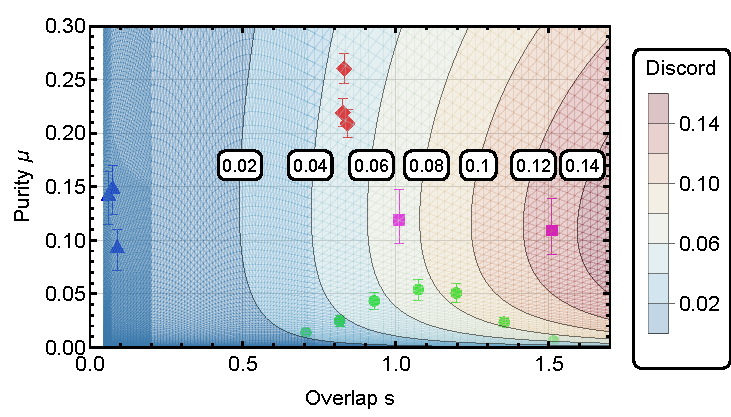
\includegraphics[scale=1.0]{figure_purity_discord.pdf}
    \caption[Fig3]{\textbf{Two-dimensional state purity $\mu$ for the motion of a nanoparticle in the tweezer transverse plane.} We show the results obtained in different experiments, as a function of the overlap parameter $\supp = 2 (\gX^2+\gY^2)/\kappa \delta$. Green dots: Ref. \cite{Ranfagni2022}. Magenta squares: Ref. \cite{Ranfagni2023}. Blue triangles: Ref. \cite{Piotrowski2023}. Red diamonds: this work, including the additional data sets \cite{SM1}. In order to provide an indication of the two-dimensional correlations present in the mechanical system, we also show the contour plot of the symmetrized quantum discord $0.5 (\mathcal{D}_{X \leftarrow Y} + \mathcal{D}_{Y \leftarrow X})$, calculated with the following parameters: $\gX/2\pi = \gY/2\pi = 12400$ Hz,  $\GX/2\pi = \GY/2\pi$ varying between 100 Hz and 300 kHz, $\Delta = -0.5(\OmegaX+\OmegaY)$. The other parameters are chosen similar to those of the present work for $\supp >  0.7$, while for $\supp < 0.7$ they change to keep realistic ranges. In details, for $\supp > 0.7$ we use $\kappa/2\pi = 57$ kHz and $(\OmegaX+\OmegaY)/4\pi = 116$ kHz. For $\supp < 0.7$ both the cavity width and the mean oscillation frequency increase, reaching $\kappa/2\pi = 330$ kHz and $(\OmegaX+\OmegaY)/4\pi = 246$ kHz when $\supp = 0.07$, thus approaching the parameters of \cite{Piotrowski2023}. The variations laws are $\kappa/2\pi = [57 + (330-57)x^4]\,\mathrm{kHz}$ and $(\OmegaX+\OmegaY)/4\pi = [116 + (246-116)x^2]\,\mathrm{kHz}$ where $x = (\supp - 0.7)/(0.07 - 0.7)$. In the full graph, the frequency splitting $\delta$ is determined by $\supp$ according to $\supp = 2 (\gX^2+\gY^2)/\kappa \delta$.}
    \label{Fig3}
\end{figure}

The relevance of the correlation between the $X$ and $Y$ projections of the two-dimensional motion can be quantified by the quantum discord $\mathcal{D}_{X \leftarrow Y}$ ($\mathcal{D}_{Y \leftarrow X}$), defined as the difference between the mutual information between the two subsystems, and the one-way classical correlations. The latter is the maximum amount of information obtainable on $X$ ($Y$) by locally measuring the sub-system $Y$ ($X$). A positive discord, even on separable (not entangled) states, is an indicator of quantumness \cite{Ollivier2002}. For bipartite Gaussian states, the expression of the quantum discord can be written in a close form using the four symplectic invariants of the covariance matrix \cite{Giorda2010,Adesso2010,Olivares2012}. We obtain $\mathcal{D}_{X \leftarrow Y} = 0.0423\pm0.0007$ and $\mathcal{D}_{Y \leftarrow X} = 0.0471\pm0.0012$. A contour plot of the symmetrized discord $0.5 (\mathcal{D}_{X \leftarrow Y} + \mathcal{D}_{Y \leftarrow X})$ is displayed in Fig. \ref{Fig3} showing that, as expected, a larger quantum discord is achieved at increasing spectral overlap. Even if a small but positive discord can exist even for states with low purity, and it is indeed a rather general feature \cite{Ferraro2010}, in our case the discord constitutes a sizeable part of the total mutual information, roughly half of it, so quantum correlations are of the same order as total correlations. 

The description based on the original $X$ and $Y$ modes does not capture the full physical properties of the optomechanical system. As $\splitt$ decreases, the motion is better understood using a description based on the geometric bright and dark modes, corresponding to directions parallel and orthogonal to the cavity axis, respectively. With this basis, it has been shown that the two-dimensional cooling becomes less effective since the dark mode is not directly coupled to the optical field. Moreover, as the strong optomechanical coupling is approached, optical cooling becomes less efficient as it assumes a sublinear dependence on $g^2$. As an additional effect of strong coupling, the identification of two orthogonal oscillation directions as approximate eigenvectors of the complete optomechanical system becomes poorly accurate~\cite{Ranfagni2021}. We derive two considerations. 
The first is that, for a fair description of the system, we need to abandon the ($X-Y$) coordinate system, and prioritize indicators that are independent of any specific reference frame. The global state purity already satisfies this requirement. For quantum discord, we evaluated the maximum of $\,\mathcal{D}_{\phi \,\leftarrow (\phi+\pi/2)} $ where $\phi$ defines the projection of the two-dimensional motion along the $\phi$ direction. We obtain a value of $0.0482\pm0.0012$ for an angle $\phi = -9^{\circ}$.
The second consideration is that simultaneously achieving a low effective temperature (i.e., high state purity) and large spectral overlap (i.e., strongly two-dimensional characteristics) is not obvious. Appropriate tuning of the system parameters allows one to maximize either the purity or the discord, and the quantum indicators pair can thus be optimized for specific applications. 



\section*{Conclusions}
 
In conclusion, we have achieved two-dimensional motion of a nanosphere in an optical potential where not only the oscillations predominantly occupy the quantum ground state in all directions across the plane, setting a new benchmark for the purity of the two-dimensional state, but also significant correlations are consistently present between any pair of orthogonal directions.
Therefore, the system behavior cannot be reduced to a simple decomposition into two one-dimensional modes. Instead, the motion exhibits distinct two-dimensional characteristics that can be detected spectrally.

The measured correlations are not yet strong enough to produce entanglement between mechanical modes (i.e., between oscillations along two directions of the plane). In fact, it has been shown theoretically that achieving this type of entanglement is almost impossible with our setup in its present configuration, where the background is at room temperature and only a single mode of the electromagnetic field is present \cite{Vitali2007,Genes2008}. However, the system we have developed, characterized by high purity and strong spectral correlations, represents an excellent platform for achieving entanglement, for example by introducing additional electromagnetic fields \cite{Hartmann2008,Li2015}. By adding blue-detuned laser fields to the tweezer light, with a controlled phase relationship with respect to the cooling radiation, one could implement schemes similar to those successfully realized in ultra-cryogenic microwave experiments, where entanglement between oscillators quadratures is achieved \cite{Ockeloen-Korppi2018,Kotler2021,Mercier2021}. Furthermore, as proposed in Ref. \cite{Mazzola2011}, an additional cavity would allow to activate entanglement between the two mechanical oscillators exhibiting quantum discord. Pulsed schemes where the entangling fields enter the cavity through its output port are also promising \cite{Rakhubovsky2020}.
The realization of mechanical entanglement would mark a significant milestone in the development of innovative quantum information schemes \cite{Weedbrook2012}, as well as for the study of quantum decoherence at the macroscopic level \cite{Marshall2003,Bassi2013,Gasbarri2021}.

\section*{Acknowledgments}
We acknowledge financial support from PNRR MUR Project No. PE0000023-NQSTI and by the European Commission-EU under the Infrastructure I-PHOQS “Integrated Infrastructure Initiative in Photonic and Quantum Sciences ” [IR0000016, ID D2B8D520, CUP D2B8D520].




\bibliography{database}




%\bibliographystyle{apsrev4-2} 
%\bibliography{database}



\end{document}